\section{Psicologia Humanista}\label{humanismo}

Os principais idealizadores são Abraham Maslow~(1908-1970) e Carl Rogers~(1902-1987), tendo o apogeu desta escola as décadas de 1950 e 1960. 
O que fomentou o humanismo foi a insatisfação na qual a escola Behaviorismo e a Psicanálise abordavam o ser humano. 
Assim, a psicologia humanista fundamenta e defende a pessoa como o centro de estudo, não o seu comportamento, de modo a ressaltar a liberdade do homem, isto é, as suas vontade, o desenvolvimento pessoal e a auto-realização, em oposição ao controle como é feito pelo Behaviorismo.
Também critica a psicanálise, pois defende que os seres humanos são seres conscientes e enfatiza a espontaneidade e o papel do criador do ser humano~\cite{silva2007psicologia_educacao}.
Portanto, a psicologia humanista possui o objetivo em ajudar as pessoas a alcançar e realizar o seu potencial e finalmente a auto-realização, que é expressa pela Hierarquia das necessidades de Maslow \cite{laruse2009geral,rogers2017pessoa}, vide a Figura~\ref{img:triangulo-maslow}, a ilustração foi realizado por J. Finkelstein~\footnote{https://commons.wikimedia.org/wiki/User:J.\underline{\hspace{.1cm}}Finkelstein} e traduzida para o idioma português por Felipe Sanches~\footnote{https://pt.wikipedia.org/wiki/Ficheiro:Hierarquia\underline{\hspace{.1cm}}das\underline{\hspace{.1cm}}necessidades\underline{\hspace{.1cm}}de\underline{\hspace{.1cm}}Maslow.svg}.


\begin{figure}[!htp]
    \centering
    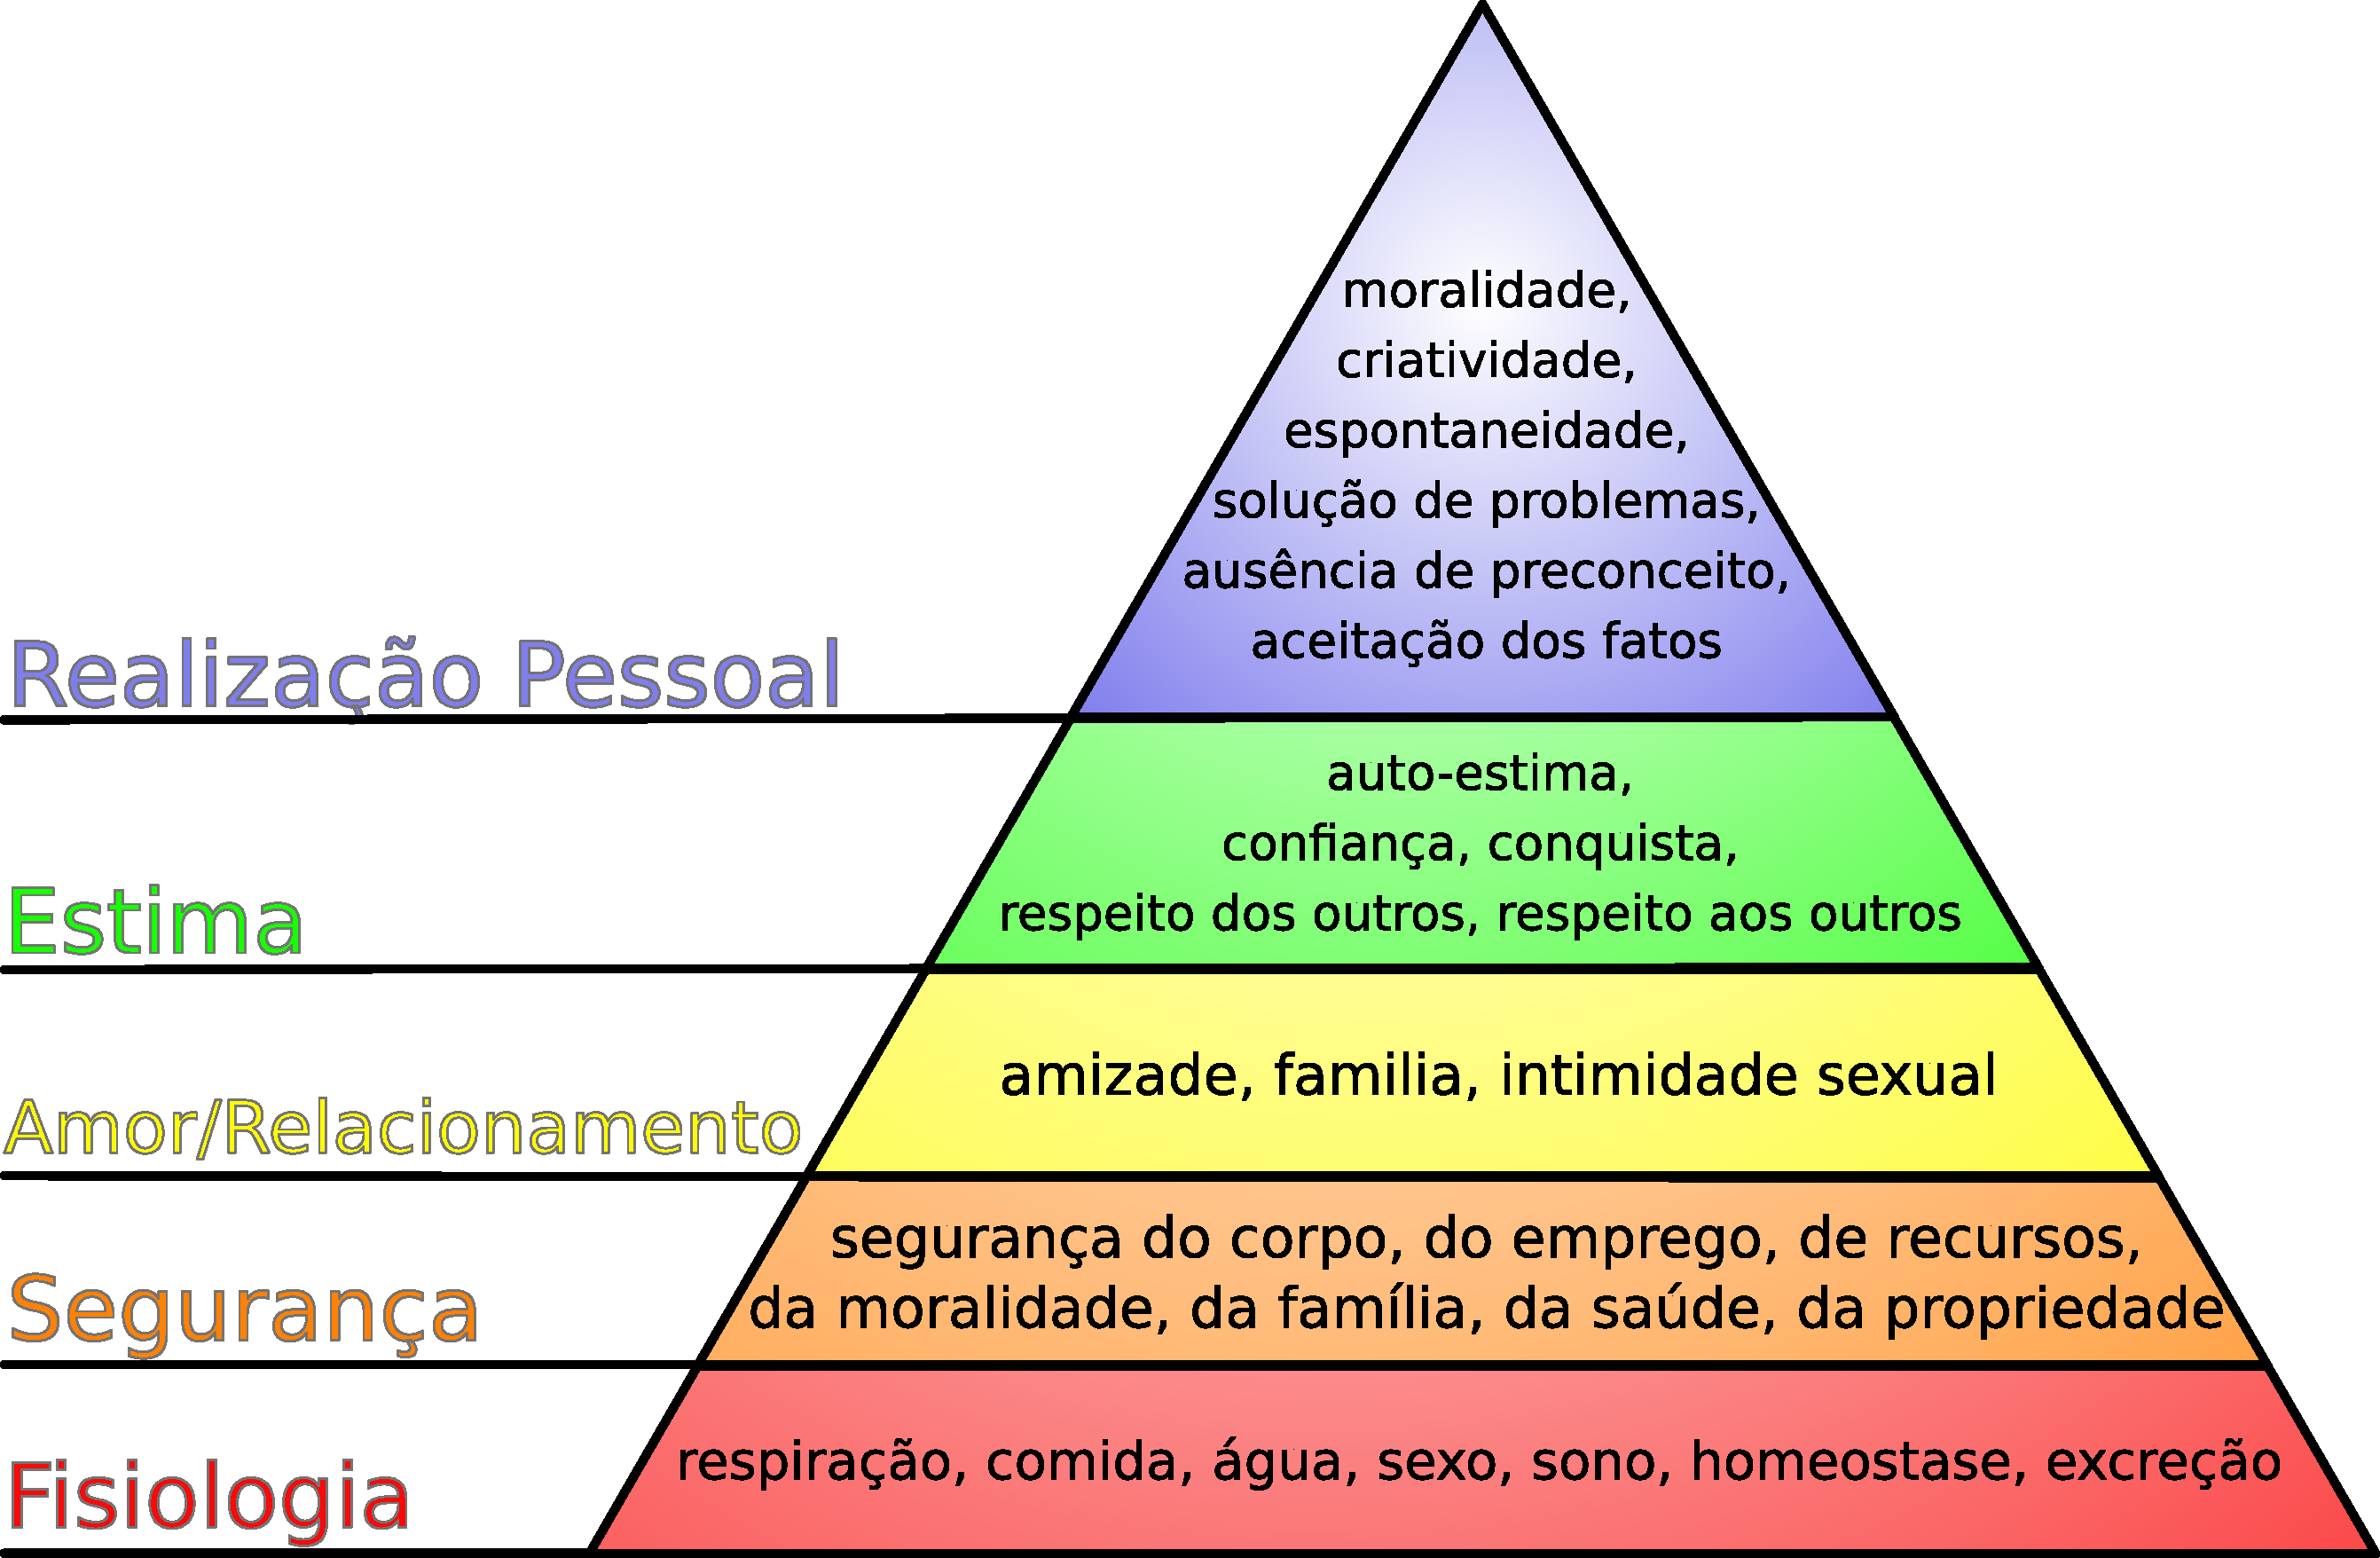
\includegraphics[scale=.32]{../../../img/psicologia/triangulo-maslow.pdf}
    \caption{
                Hierarquia das necessidades de Maslow. 
                Fonte: J. Finkelstein traduzida por Felipe Sanches, tendo a licença Creative Commons da Wikimedia Commons.
            }
    \label{img:triangulo-maslow}
\end{figure}


O principal fator promotor do desenvolvimento da personalidade é uma tendência inata dos seres humanos para a auto-realização. 
As pessoas que vivem todo o seu potencial são aquelas que vivem plenamente a cada momento, deixando-se guiar por seus próprios instintos, em lugar de levar em consideração opiniões alheias. 
Assim, as pessoas de pensamento livre e alta criatividade.
Também defendeu o autoconceito como um padrão organizado e consciente das características de cada um desde a infância, à medida que novas experiências surgem, os conceitos podem ser substituídos ou reforçados. 
Destarte, a capacidade do indivíduo de modificar consciente e racionalmente seus pensamentos e comportamentos, fornece a base para a formação de sua personalidade. 

A teoria da motivação desenvolvida por Maslow tendo o intuito de provar que as necessidades humanas são organizadas em hierarquia, pois tal hierarquia guia o ser humano em seu desenvolvimento para satisfazer as necessidades ao decorrer da vida, tais necessidades é representada na Figura~\ref{img:triangulo-maslow}, o qual o homem se movimenta dentro da hierarquia de acordo com as necessidades, assim que são sanadas ele avança, há também possibilidade de regresso.
Destarte, as necessidades são guiadas pelo comportamento do próprio indivíduo ou de fatores externos, tendo o objetivo de alcançar o nível mais alto da hierarquia, sendo a meta a realização pessoal, não obstante nem todos alcançam tal deleito~\cite{laruse2009geral}.

Abordagem centrada na pessoa desenvolvida por Carl Rogers, no qual defende o desenvolvimento da personalidade é inata aos seres humanos, bem como a pessoas que almejam ou alcançam a auto-realização são guiados pela vontade consciente e não por opiniões alheias, isto é, o ser humano é espontâneo, por conseguinte o homem está em constante evolução, não podendo ser rotulado em um esquema de modo reducionista, pois ele é possui a habilidade de enfrentar e adaptar às adversidades, sendo ser dotado de característica antifrágil, denominada por Rogers de tendência atualizante~\cite{rogers2017pessoa}. 

A psicologia humanista continua influenciando o estudo da psicologia, principalmente o campo da psicologia positiva, que visa em contribuir com a auto-realização da pessoa tendo a finalidade de tornar a vida dessa mais prazerosa, feliz, gratificante e agradável, ou seja, melhorar a qualidade de vida e pessoal do ser humano envolvidos por esta abordagem humanista. 
